%% 
%% Copyright 2007-2025 Elsevier Ltd
%% 
%% This file is part of the 'Elsarticle Bundle'.
%% ---------------------------------------------
%% 
%% It may be distributed under the conditions of the LaTeX Project Public
%% License, either version 1.3 of this license or (at your option) any
%% later version.  The latest version of this license is in
%%    http://www.latex-project.org/lppl.txt
%% and version 1.3 or later is part of all distributions of LaTeX
%% version 1999/12/01 or later.
%% 
%% The list of all files belonging to the 'Elsarticle Bundle' is
%% given in the file `manifest.txt'.
%% 
%% Template article for Elsevier's document class `elsarticle'
%% with numbered style bibliographic references
%% SP 2008/03/01
%% $Id: elsarticle-template-num.tex 272 2025-01-09 17:36:26Z rishi $
%%
%\documentclass[preprint,12pt]{elsarticle}

%% Use the option review to obtain double line spacing
\documentclass[authoryear,preprint,review,12pt]{elsarticle}

%% Use the options 1p,twocolumn; 3p; 3p,twocolumn; 5p; or 5p,twocolumn
%% for a journal layout:
%% \documentclass[final,1p,times]{elsarticle}
%% \documentclass[final,1p,times,twocolumn]{elsarticle}
%% \documentclass[final,3p,times]{elsarticle}
%% \documentclass[final,3p,times,twocolumn]{elsarticle}
%% \documentclass[final,5p,times]{elsarticle}
%% \documentclass[final,5p,times,twocolumn]{elsarticle}

%% For including figures, graphicx.sty has been loaded in
%% elsarticle.cls. If you prefer to use the old commands
%% please give \usepackage{epsfig}

%% The amssymb package provides various useful mathematical symbols
\usepackage{amssymb}
%% The amsmath package provides various useful equation environments.
\usepackage{amsmath}


\usepackage{hyperref}
\usepackage[english]{babel}
\usepackage[utf8]{inputenc}
\usepackage[T1]{fontenc}
\usepackage{subcaption}


\bibliographystyle{elsarticle-harv}

%% The amsthm package provides extended theorem environments
%% \usepackage{amsthm}

%% The lineno packages adds line numbers. Start line numbering with
%% \begin{linenumbers}, end it with \end{linenumbers}. Or switch it on
%% for the whole article with \linenumbers.
\usepackage{lineno}

\journal{Pattern Recognition Letters}


%% Mathematical Notation

%%%%%%%%%%%%%%% COMMENTAIRES %%%%%%%%%%%%%%%

\newcommand{\CA}[2]{\textcolor{gray}{#1}\textcolor{orange}{\quad #2}}
\newcommand{\ms}[1]{\textcolor{cyan}{#1}}
\newcommand{\MS}[2]{\textcolor{cyan}{#1}\textcolor{teal}{\quad #2}}
\newcommand{\kds}[2]{\textcolor{orange}{#1}\textcolor{red}{\quad #2}}

%%%%%%%%%%%%%%% VARIABLES MATHEMATIQUES %%%%%%%%%%%%%%%

\DeclareMathOperator{\indep}{\perp \!\!\! \perp}
\DeclareMathOperator{\ind}{\mathds{1}}
\DeclareMathOperator{\dir}{\text{Dir}}
\DeclareMathOperator{\bet}{\text{Beta}}
\DeclareMathOperator{\KL}{\textbf{KL}}
\DeclareMathOperator{\1}{\mathds{1}}
\DeclareMathOperator{\p}{\mathbb{P}}
\DeclareMathOperator{\M}{\mathcal{M}}
\DeclareMathOperator{\argmin}{\arg\!\min}
\DeclareMathOperator{\argmax}{\arg\!\max}
\DeclareMathOperator{\diag}{\operatorname{diag}}

\newcommand{\bA}{\mathbf{A}}
\newcommand{\bX}{\mathbf{X}}
\newcommand{\bZ}{\mathbf{Z}}
\newcommand{\bW}{\mathbf{W}}
\newcommand{\by}{\mathbf{y}}
\newcommand{\bG}{\mathbf{G}}
\newcommand{\bTheta}{\mathbf{\Theta}}
\newcommand{\bpi}{\boldsymbol{\pi}}
\newcommand{\brho}{\boldsymbol{\rho}}
\newcommand{\bbeta}{\boldsymbol{\beta}}
\newcommand{\balpha}{\boldsymbol{\alpha}}
\newcommand{\bgamma}{\boldsymbol{\gamma}}
\newcommand{\softmax}{\operatorname{softmax}}

\newcommand{\dataset}{{\cal D}}
\newcommand{\Xspace}{{\cal X}}
\newcommand{\E}{{\mathbb{E}}}
\newcommand{\fracpartial}[2]{\frac{\partial #1}{\partial  #2}}
\newcommand\flowsfroma{\mathrel{\vcenter{\hbox{\rotatebox{180}{$\leadsto$}}}}}

\usepackage{breqn}




\begin{document}

\begin{frontmatter}

%% Title, authors and addresses

%% use the tnoteref command within \title for footnotes;
%% use the tnotetext command for theassociated footnote;
%% use the fnref command within \author or \affiliation for footnotes;
%% use the fntext command for theassociated footnote;
%% use the corref command within \author for corresponding author footnotes;
%% use the cortext command for theassociated footnote;
%% use the ead command for the email address,
%% and the form \ead[url] for the home page:
%% \title{Title\tnoteref{label1}}
%% \tnotetext[label1]{}
%% \author{Name\corref{cor1}\fnref{label2}}
%% \ead{email address}
%% \ead[url]{home page}
%% \fntext[label2]{}
%% \cortext[cor1]{}
%% \affiliation{organization={},
%%             addressline={},
%%             city={},
%%             postcode={},
%%             state={},
%%             country={}}
%% \fntext[label3]{}

\title{Conditional Latent Block gated Mixture of Experts}

\author[affilation1]{De Santiago, Kylliann} %% Author name
\author[affilation1]{Ambroise, Christophe} %% Author name
\author[affilation1]{Szafranski, Marie} %% Author name

    
\affiliation[affiliation1]{organization={LaMME, UMR CNRS 8071, University of Paris-Saclay},
             addressline={23 boulevard de France},
city={Evry},
postcode={91000},
state={},
country={France}}

%% Abstract
\begin{abstract}
A key advantage of Mixture of Experts (MoE) is their capability for data stratification, enabling the identification and characterization of subpopulations by forming distinct communities. This is achieved through a gating network that dynamically assigns observations to specialized experts. However, a notable limitation of MoE models is their potential to function as black boxes, making variable interpretation challenging . The complexity of interpretation is influenced by the type of gating network and expert models employed.

We introduce an interpretable MoE framework that not only characterizes subpopulations but also captures the redundancy and complementarity of information specific to each community. To achieve this, we propose extending MoE models by incorporating a conditional biclustering structure as a gating network. This approach leads to interpretable MoEs that reveal the redundancy and complementarity of information by clustering variables into components. Additionally, this fusion enhances computational efficiency by allowing specialized experts to focus on the redescription of variables, with representative variables characterizing the components.
\end{abstract}

%%Graphical abstract
\begin{graphicalabstract}
\begin{figure}[!ht]
     \centering
     \begin{subfigure}[b]{\textwidth}
         \centering
         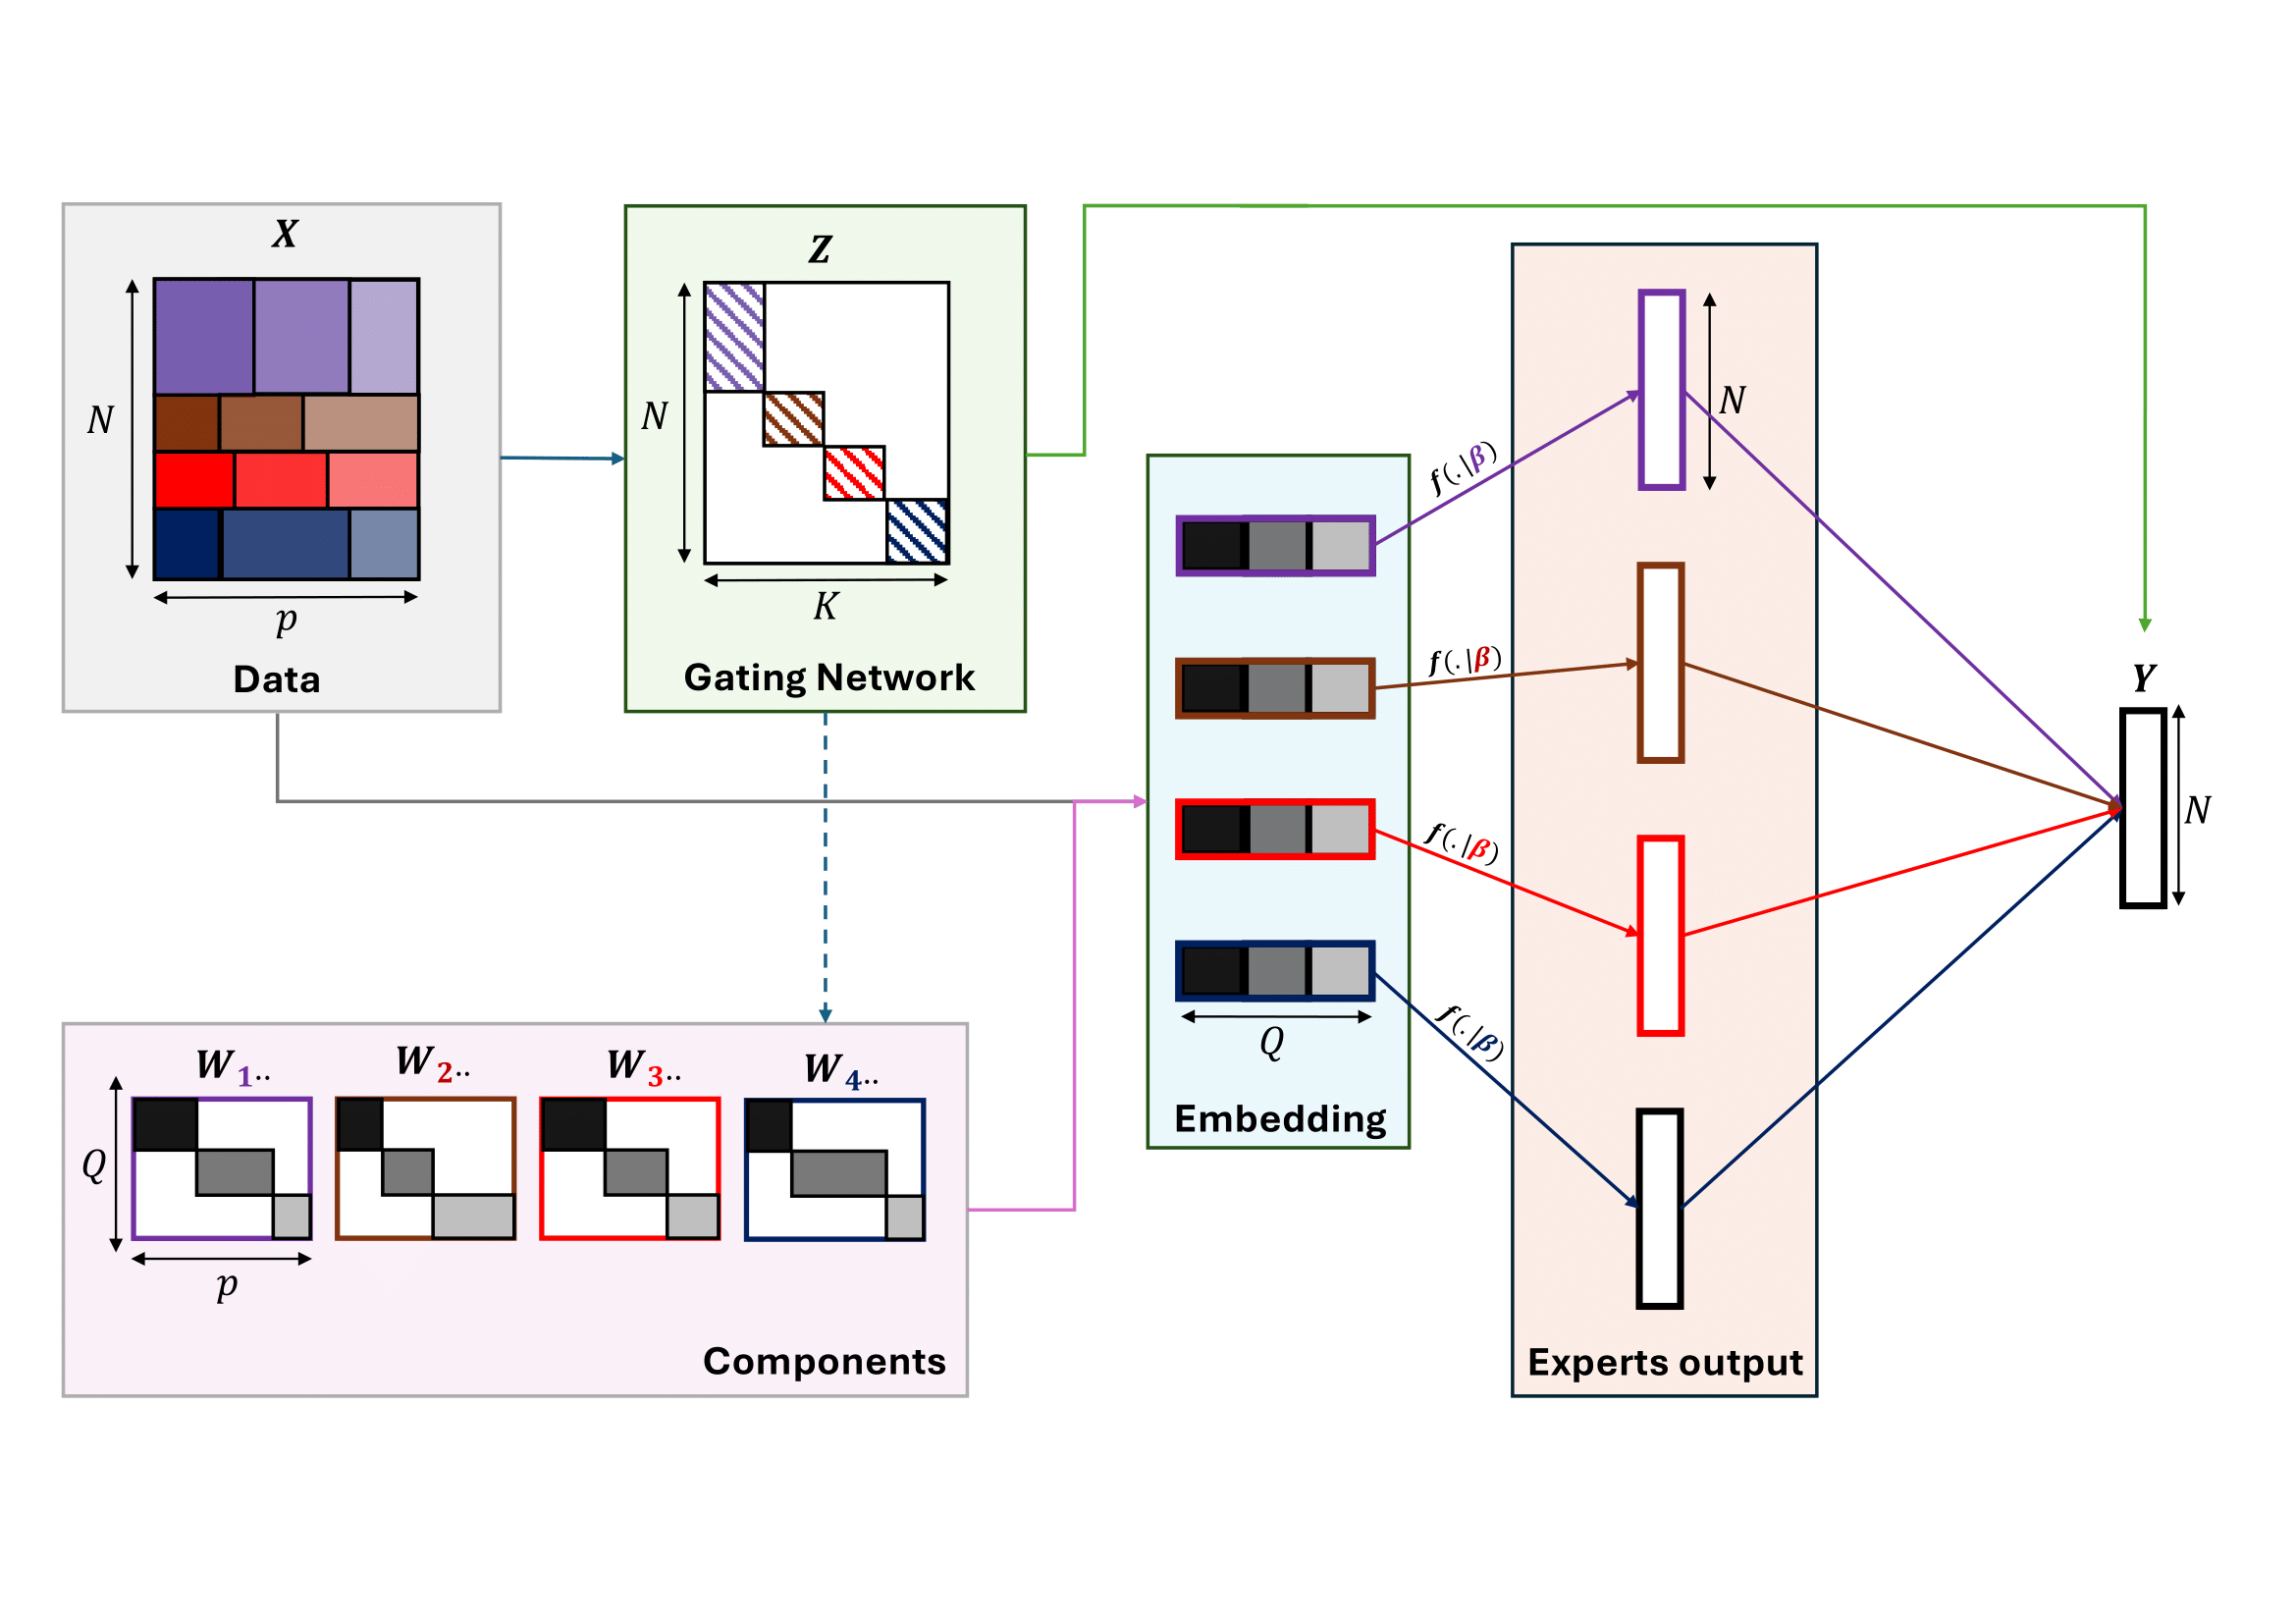
\includegraphics[width=\textwidth]{Figures/CocoLBMoE.png}
     \end{subfigure}
     \hfill
     \caption{ Schematic representation of \textit{MoEBIUS}.
     The input data \( \bX \), of dimension \( N \times p \), is used to define selection weights for the $K$ experts (gating network $\bZ$, with $K$ communities).
     Each expert is associated with a projection matrix \( \bW_k \), of dimension \( p \times Q \), that groups the covariates into components. The data, coupled with the projection matrices, are transformed into matrices of size \( N \times Q \), which are then passed through a regression function \( f_k(. \mid \bbeta_k) \) specific to each expert. 
     The outputs of the experts are combined according to the gating network's weights (based on community membership) to produce a final prediction \( \by \), representing the target variable.}
     \label{fig: CocoLBMoE}
\end{figure}
\end{graphicalabstract}

%%Research highlights
\begin{highlights}
    \item \textbf{Structured Expert Assignment:} The gating network is enhanced with a conditional latent block model, allowing it to group variables into coherent components. This leads to more interpretable expert assignments.
    \item \textbf{Redundancy Reduction:} By clustering correlated features, MoEBIUS minimizes redundant information, improving both computational efficiency and model generalization.
    \item \textbf{Improved Predictive Performance:} The integration of latent block models refines expert specialization, leading to higher accuracy in predictive tasks.
\end{highlights}

%% Keywords
\begin{keyword}
%% keywords here, in the form: keyword \sep keyword

%% PACS codes here, in the form: \PACS code \sep code

%% MSC codes here, in the form: \MSC code \sep code
%% or \MSC[2008] code \sep code (2000 is the default)
Mixture of Experts \sep Latent Block Model \sep Explainability
\end{keyword}

\end{frontmatter}

\section{Introduction}


Since its introduction more than two decades ago \citep{jacobs1991adaptive}
Mixture of Experts (MoE) models have been widely used in machine learning due to their ability to partition data into meaningful subpopulations and assign specialized models to different regions of the input space. 

Different types of expert
architectures have been proposed, such as SVMs \citep{Collobert2002}, Gaussian Processes \citep{Tresp2001, Theis2015, Deisenroth2015}, Dirichlet Processes \citep{Shahbaba2009},
and deep networks.

These models rely on a gating function that dynamically assigns observations to experts, allowing for adaptive learning across heterogeneous datasets. 

Conventional MoE models face challenges in interpretability. MoE models can act as black boxes, making it difficult to extract meaningful insights into how experts contribute to predictions.

To address these issues, we propose the MoEBIUS algorithm, which incorporates a conditional latent block structure into the traditional MoE framework. The key contributions of MoEBIUS are:
\begin{itemize}
    \item \textbf{Structured Expert Assignment:} The gating network is enhanced with a conditional latent block model, allowing it to group variables into coherent components. This leads to more interpretable expert assignments.
    \item \textbf{Redundancy Reduction:} By clustering correlated features, MoEBIUS minimizes redundant information, improving both computational efficiency and model generalization.
    \item \textbf{Improved Predictive Performance:} The integration of latent block models refines expert specialization, leading to higher accuracy in predictive tasks.
\end{itemize}

The remainder of this paper is structured as follows: Section 2 is a background section presenting the  context of Mixture of Experts  and how our proposal relates to other close work,  Section 3 discusses the methodology and formalizes the MoEBIUS model.  
Section 4 provides experimental validation, comparing MoEBIUS against standard MoE approaches. Finally, Section 5 concludes with a discussion on potential applications and future research directions.

\section{Background and related work}




In Mixture of Experts, although each expert receives all input variables, only a subset is truly relevant to the specific task assigned to the expert. This variable selection is frequently implicit, as each expert focuses on the most useful characteristics for its task. However, this selection can be made explicit through regularization mechanisms, such as $L_1$ \citep{courbariaux2022sparse}, $L_2$ \citep{jordan1994hierarchical}, or elastic net \citep{chamroukhi2019regularized, ma2018modeling}. For $K$ experts, this would be equivalent %to trying 
to maximize the following quantity:
%
\begin{align}
    \mathcal{L}(\bbeta,\bpi ; \by,\bX) &= \prod_{i=1}^N \sum_{k=1}^K \underbrace{g\left(\bX_i ; \bpi \right)_k}_{\text{Gating Network}}
   \underbrace{ f_k\left(y_i; \bX_i, \bbeta_k\right)}_{\text{Expert}} \notag
   \\ &\quad + \underbrace{\lambda \left( \alpha \sum_{k=1}^K \sum_{j=1}^p \lvert \pi_{kj} \rvert  + \dfrac{1-\alpha}{2}\sum_{k=1}^K \sum_{j=1}^p \pi_{kj}^2\right) }_{\text{Regularization terms}},
    %\sum_{\bZ \in \mathcal{Z}} \prod_{i=1}^N  \p\left(Z_i \mid \bX_i \right) \p\left( y_i \mid Z_i, \bX_i \right) & (probabilist modeling)
\end{align}
%
where $g\left(\bX_i ; \bpi \right)_k$ is the $k$-th output of the gating network detailed in Equation~\eqref{eq:g_k}, $\bpi$ are gating network parameters, $(\bbeta_k)_{k=1:K}$ are experts parameters, $\lambda>0$ is an hyperparameter linked to regularization strength and $\alpha>0$ is an hyperparameter for elastic-net regularization.

These regularizations, primarily applied to the gating network, enhance interpretability by controlling expert selection directly. The gating network plays a central role in variable and expert selection, and different approaches can be classified into three main categories \cite{cai2024survey}: dense \citep{wu2023mole, pan2024dense}, sparse \citep{jiang2024mixtral, tan2023sparse, zhou2022mixture}, and soft \citep{puigcerver2023sparse, zadouri2023pushing}. 

In sparse methods, regularizations are designed to activate a limited number of experts or variables, which improves the interpretability by aligning predictions with the variables involved \citep{zhou2022mixture}. 
The main approach is to use the top-$L$ experts, meaning the $L$ experts with the highest values according to the gating network:
%
in general, the gating network $g$ is composed of $(g_k)_{k=1:K}$ functions, and is defined as
\begin{equation}
    g(\bX_i ; \bpi) = \softmax \left(g_1\left(\bX_i ; \bpi_1 \right), \cdots, g_K\left(\bX_i ; \bpi_K \right) \right). 
\end{equation}
Typically, to limit the number of activated experts, according to \cite{cai2024survey}, the gating network output $g(\bX_i)_k$ is replaced by:
\begin{equation}
\label{eq:g_k}
    \tilde{g}(\bX_i)_k = \softmax\left(\operatorname{TopL}\left( g_1\left(\bX_i; \bpi_1\right) \right),\cdots,\operatorname{TopL}\left(g_K\left(\bX_i; \bpi_K\right)\right) \right)_k,
\end{equation}
where 
\begin{equation}
    \operatorname{TopL}(g_k(\bX_i; \bpi)) = \left\{
    \begin{array}{ll}
        g_k(\bX_i; \bpi) & \mbox{if } g(\bX_i; \bpi)_k \in \text{top-L elements of } g(\bX_i; \bpi), \\
        -\infty & \mbox{else.} 
    \end{array}
    \right.
\end{equation}
%
Currently, sparse MoEs typically refers to limiting the number of active experts, thereby reducing computational cost. However, an increased specialization among a large pool of experts does not necessarily ensure sparsity in terms of variable selection.
%
On the other hand, soft approaches allow more gradual and partial expert activation, offering a balance between sparsity and flexibility. 
All MoEs with regularization mechanisms on the gating network fall into this class of models. 
While these models achieve sparsity in terms of variable selection, they remain soft in terms of expert activation. Indeed, it is not always possible to ensure that only a minimal subset of experts will be activated.
%This may limit their ability to produce entirely sparse solutions in terms of the experts selected.

The integration of these penalties structures the gating network's behavior and encourages a parsimonious selection of variables. This simplifies interpretation by reducing the number of variables and experts involved in decision-making, while maintaining computational efficiency \citep{shazeer2017outrageously}. However, the separation between variables used by the gating network and those leveraged by experts in the final prediction can complicate the interpretability, as the most influential variables for selection are not always the most relevant for prediction. This disjunction introduces a potential bias in model interpretation.
Several efforts have been made to improve the interpretability of MoEs, for instance:
\begin{itemize}
    \item \cite{ismail2022interpretable} developed an interpretable MoE model, introducing an approach that makes expert decisions more transparent by employing explanation techniques such as assignment modules and studying expert contributions.
    \item Since 2017, the integration of attention mechanisms in MoEs, as presented by \cite{shazeer2017outrageously}, has made the decision process more explicit by focusing the model's attention on specific aspects of the data. Additionally, this work introduced the concept of the MoE-layer, which has been widely reused in recent Deep Learning architectures \citep{lepikhin2020gshard, fedus2022switch, zhou2022mixture}.
    \item In the context of Multitask Learning, \cite{ma2018modeling} proposed using multiple gating networks, linked to the associated prediction tasks, providing a clearer connection between the experts utilized, the gating network predictions, and the final outcomes.
\end{itemize}

Ensuring interpretability is an important aspect in machine learning applied to sensitive areas. In Mixture Of Experts framework, which can be achieved not only through the design of the gating mechanism but also by employing interpretable experts. Experts based on linear regression are a common choice in this regard, as they allow for a clear justification of the decisions made by each expert. Moreover, experts based on linear regression are often favored due to their computational efficiency.

These type of Mixture of Experts models generally fall within the category of Latent Regression Models (LRMs), where the experts are based on latent subpopulations, and the regression coefficients capture subgroup-specific effects \citep{vermunt2002latent, desarbo1988maximum}.
More specifically, the general model is often defined as follows:
\begin{align}
    \bZ_i &\sim \M\left(1; \bpi = \left(\pi_1, \cdots, \pi_K\right) \right), \\
    y_i \mid \bX_i, Z_{ik}=1 &\sim \mathcal{N}\left(\bX_i \bbeta_k, \sigma^2_k\right),
\end{align}
where $\bZ_i$ is a latent variable for expert allocation for observation $i$ and $\bbeta_k$ are regression parameters for the $k$-th expert (or community).

In this framework, the role of the gating network is associated with the variable $Z$. This variable refers to community membership, it is assumed that individuals from the same cluster are studied by the same expert.


Nevertheless, several extensions have been developed, including longitudinal data models and co-clustering regression models.

\paragraph{Longitudinal data models:} Individuals within the same community share similar dynamics over time. Each latent class has its own risk profile for the event under study or its own longitudinal pattern \citep{proust2014joint, courbariaux2022sparse}.
Following the model of \cite{courbariaux2022sparse}, and with our notations, we would have :
\begin{align}
    \bZ_i &\sim \M\left(1; \softmax\left(\bX_i \bpi \right)\right), \\
    y_{iv} \mid \bX_i, \mathbf{T}_i, Z_{ik}=1 &\sim \mathcal{N}\left( \sum_{r=1}^R  \beta_{kvr} T_{iv}^r , \sigma^2_{vk}\right).
\end{align}
In this context, $\bX$ is considered as a $N \times p$ matrix. The latent variable is obtained by a multiclass regression parameterized  by a $p \times K$ matrix $\bpi$.
On the $v$-th visit and for the community $k$, the polynomial regression is parameterized by $\bbeta_{kv}$, and $T_{iv}$ is the time metric (the
patient’s age or time since the disease was first diagnosed, for instance).
 
\paragraph{Co-clustering Regression Model:} \cite{vu2015variational} proposed a multitask regression algorithm based on an \textit{LBM} partitioning of the $N \times p$ label matrix $\mathbf{y}$.
Each block of the matrix is associated with regression parameters for the covariates $\bX$. The Latent Block Regression Model (\textit{LBRM}) developed by \cite{boutalbi2022latent} extends this by partitioning the $N \times p \times d$-tensor $\bX$ based on the same stratification as the label matrix $\mathbf{y}$. The last dimension of the tensor $\bX$ corresponds to the covariates used in the regression.
More precisely, and with our notations :
%
\begin{align}
    \bZ_i &\sim \M\left(1; \bpi = \left(\pi_1, \cdots, \pi_K\right) \right), \\
    \bW_j &\sim \M\left(1; \brho = \left(\rho_1, \cdots, \rho_Q\right) \right), \\
    y_{ij} \mid \bX_{ij}, Z_{ik}=1, W_{js}=1 &\sim \mathcal{N}\left(\bX_{ij} \bbeta_{ks}, \sigma^2_{ks}\right).
\end{align}
 For an observation \( i \) belonging to community \( k \) and a problem \( j \) in category \( s \), a regression is performed along the third dimension, on $(\bX_{ijr})_{r=1:d}$, parameterized by a coefficient vector \( \bbeta_{ks} \in \mathbb{R}^d \).

In the supervised framework, we aim to achieve both interpretability and predictive performance. The objective of our approach is to incorporate an additional structure into the data used for prediction. While the stratification of individuals is already induced by the Mixture of Experts framework, we aim to extend this by also integrating a structure on the variables. Through a mixture model applied to covariates, the goal is to capture the emergence of both redundant information within components and complementary information between components. This approach mirrors the work on \textit{mimi-SBM}, which handles similar challenges but for multi-view clustering.

As illustrated in Figure \ref{fig: CoCoLBM_MNIST}, to obtain more specific partitions compared to a standard mixture model on covariates, a conditional stratification of variables, depending on the community structure, is needed. The resulting model, named Mixture Of Experts and BIclustering Unified Strategy (\textit{MoEBIUS}), merges MoEs with a conditinal biclustering algorithm to offer precise predictions alongside clear interpretation of latent communities and components.

More specifically, the model summarizes the components into a representative variable for each, then performs a regression on these representations, where the regression parameters depend on the community to which the observation belongs, an illustration of MoEBIUS is provided in Figure \ref{fig: CocoLBMoE}.

\begin{figure}[!ht]
     \centering
     \begin{subfigure}[b]{0.49\textwidth}
         \centering
         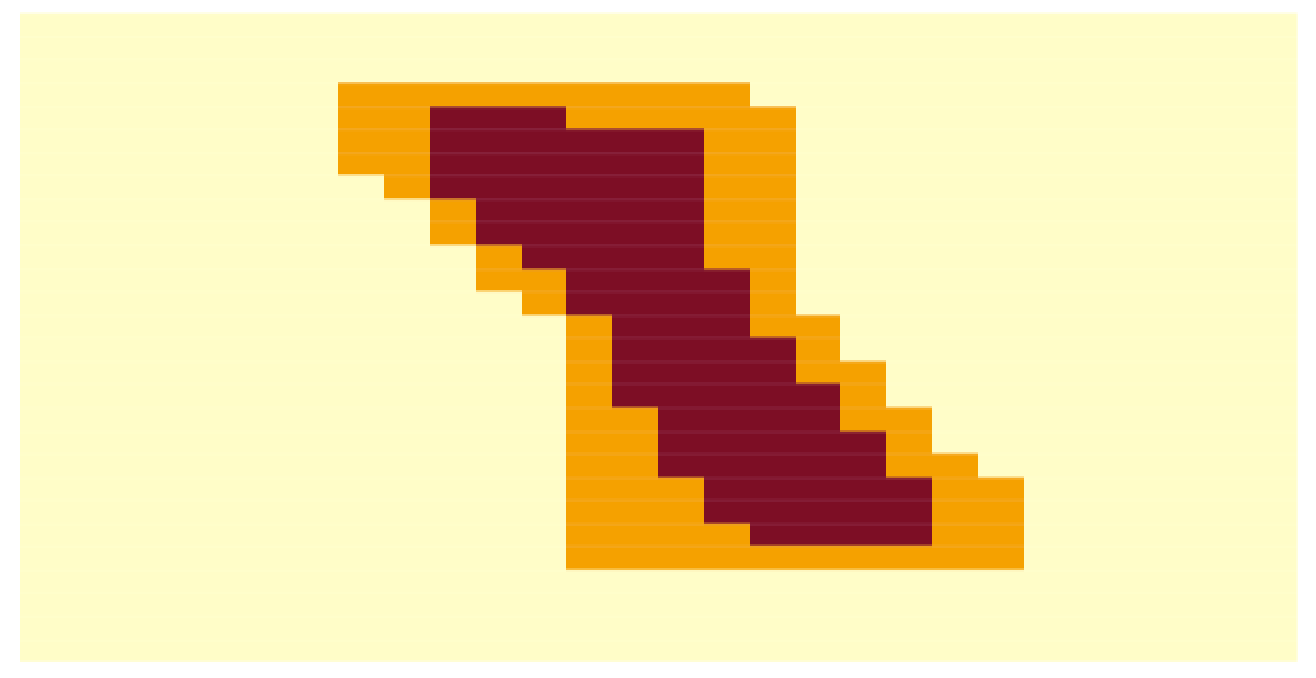
\includegraphics[width=\textwidth]{Figures/MNIST_LBM.png}
         \vspace{1.6cm}
         \caption{}
     \end{subfigure}
     \hfill
     \begin{subfigure}[b]{0.49\textwidth}
         \centering
         
\includegraphics[width=\textwidth]{Figures/MNIST_cocoLBM_1.png}
         \caption{}
         \centering
         
\includegraphics[width=\textwidth]{Figures/MNIST_cocoLBM_8.png}
         \caption{}
     \end{subfigure}
     \caption{Different component partitions on MNIST data for digits $1$ and $8$. Figure (a) shows a partition defined by an \textit{LBM}, where the overall shape of both digits is captured. Figures (b) and (c) are derived from the \textit{Conditional LBM} \citep{goffinet2020conditional}, where the partitioning of variables depends on the observations (i.e., the digits). For each partition, the key pixels of interest specific to each digit are more clearly identified.}
     \label{fig: CoCoLBM_MNIST}
\end{figure}

% \kds{
% Our approach is inspired by the work on \textit{LBRM}, aiming to partition data using a latent block model to summarize information and then applying a regression model tailored to the stratification. To obtain a finer partition than that from an LBM, we adopt the Conditional Latent Block Model approach developped by \cite[][CLBM]{goffinet2020conditional} . The combination of Mixture of Experts and biclustering algorithms has led to the development of the model presented below, named Mixture Of Experts and BIclustering Unified Strategy (\textit{MoEBIUS}).}{Dire plutôt qu'en voulant faire interpretation + perfs., partir cadre modèle d'experts, apport aspect cond. à la stratification. Remettre dans le contexte du MoEs.}



\section{MoEBIUS: Mixture of Experts and BIclustering Unified Strategy}




\subsection{Model}
MoEBIUS relies on incorporating a conditional variable stratification mechanism within Mixtures of Experts. To achieve this, we introduce a new random variable, denoted as $\bW$.
The purpose of the variable $\bW$ is to determine which covariables are considered and how they are utilized for prediction. This leads us to the following general formulation:
%
\begin{equation}
    \p\left(\by, \bW, \bZ \mid \bX, \bbeta, \brho, \bpi\right) = \underbrace{\p\left(\by \mid  \bW, \bZ,\bX, \bbeta\right)}_{\text{Experts}} 
    \underbrace{\p\left( \bW \mid \bZ, \bX, \brho\right) }_{\text{Variable stratification}} 
    \underbrace{\p\left( \bZ \mid \bX,\bpi\right)}_{\text{Gating network}}.
\end{equation}
At this stage, the specific dimensions of variables are not crucial; these details will be provided in Section \ref{sec: MoEBIUS_Model}.

The definition of experts and the law associated with \( \by \) are intrinsically dependent on the nature of the data. However, they can be formalized through a function \( f \) such that \( f(\by, \bW, \bZ, \bX, \bbeta) \), with $\bbeta$  the expert parameters.
The variable \( \bW \) is influenced by both \( \bZ \) and \( \bX \), allowing for a stratification that depends simultaneously on the communities and the individual-specific characteristics. Finally, the modeling of communities via \( \bZ \) is itself conditioned by \( \bX \); however, a marginal law could be considered.

\subsection{Mixture Of Experts and BIclustering Unified Strategy model}
\label{sec: MoEBIUS_Model}
As in \cite{courbariaux2022sparse}, the assignment to a community is obtained through a multiclass regression.
\begin{equation}
\label{eq: moebius_Z_eq}
    \bZ_{i} \mid \bX_i \sim \M\left(1; \softmax\left(\bX_i \bpi \right) \right),
\end{equation}
where $\bpi$ is a matrix of dimension $p \times K$. 

The goal is to predict the latent variable \( \bZ_+ \) for a new observation \( \bX_+ \), leveraging information obtained during model training. In this context, a regression-based approach is more appropriate than a marginal distribution, as it directly incorporates the relationships learned between the input variables and the latent variables.

Now, based on the Conditional Latent block Model (CLBM) approach developed by \cite{goffinet2020conditional}, we define the \( K \times p \times Q \) tensor \( \bW \), which models the partition of the \( p \) variables into \( Q \) components. 

These partitions are conditioned by the \( K \) communities, meaning that for each community \( k \), the partition of the variables may differ, hence introducing the conditional aspect.
%
Conditionally to the cluster $k$, each row of the component membership matrix follows: 
%
\begin{equation}
\label{eq: moebius_W_eq}
    \bW_{kj} \sim \M\left(1; \brho_k = \left(\rho_{k1},\dots,\rho_{kQ}\right) \right).
\end{equation}
One could have considered incorporating the contribution of \( \bX_i \) in the modeling process, allowing for a partition dependent on the individual rather than the community. However, this would have complicated the interpretability. The rationale behind this approach is to partially summarize the behavior of individuals through the communities to which they belong, making this modeling choice preferable.

In addition, an analysis of the effectiveness of the CLBM under the assumption of constant communities and conditional variable partitions has been conducted, through a study of the Co-Conditional Latent Block Model (\textit{Co-CoLBM}). Parameter estimation, model selection and performance on simulated data have been studied. The code is available on Github (\url{https://github.com/Kdesantiago}).
The detailed results of this study are presented in Appendix \ref{sec: CocoLBM}.


\begin{figure}[!ht]
     \centering
     \begin{subfigure}[b]{\textwidth}
         \centering
         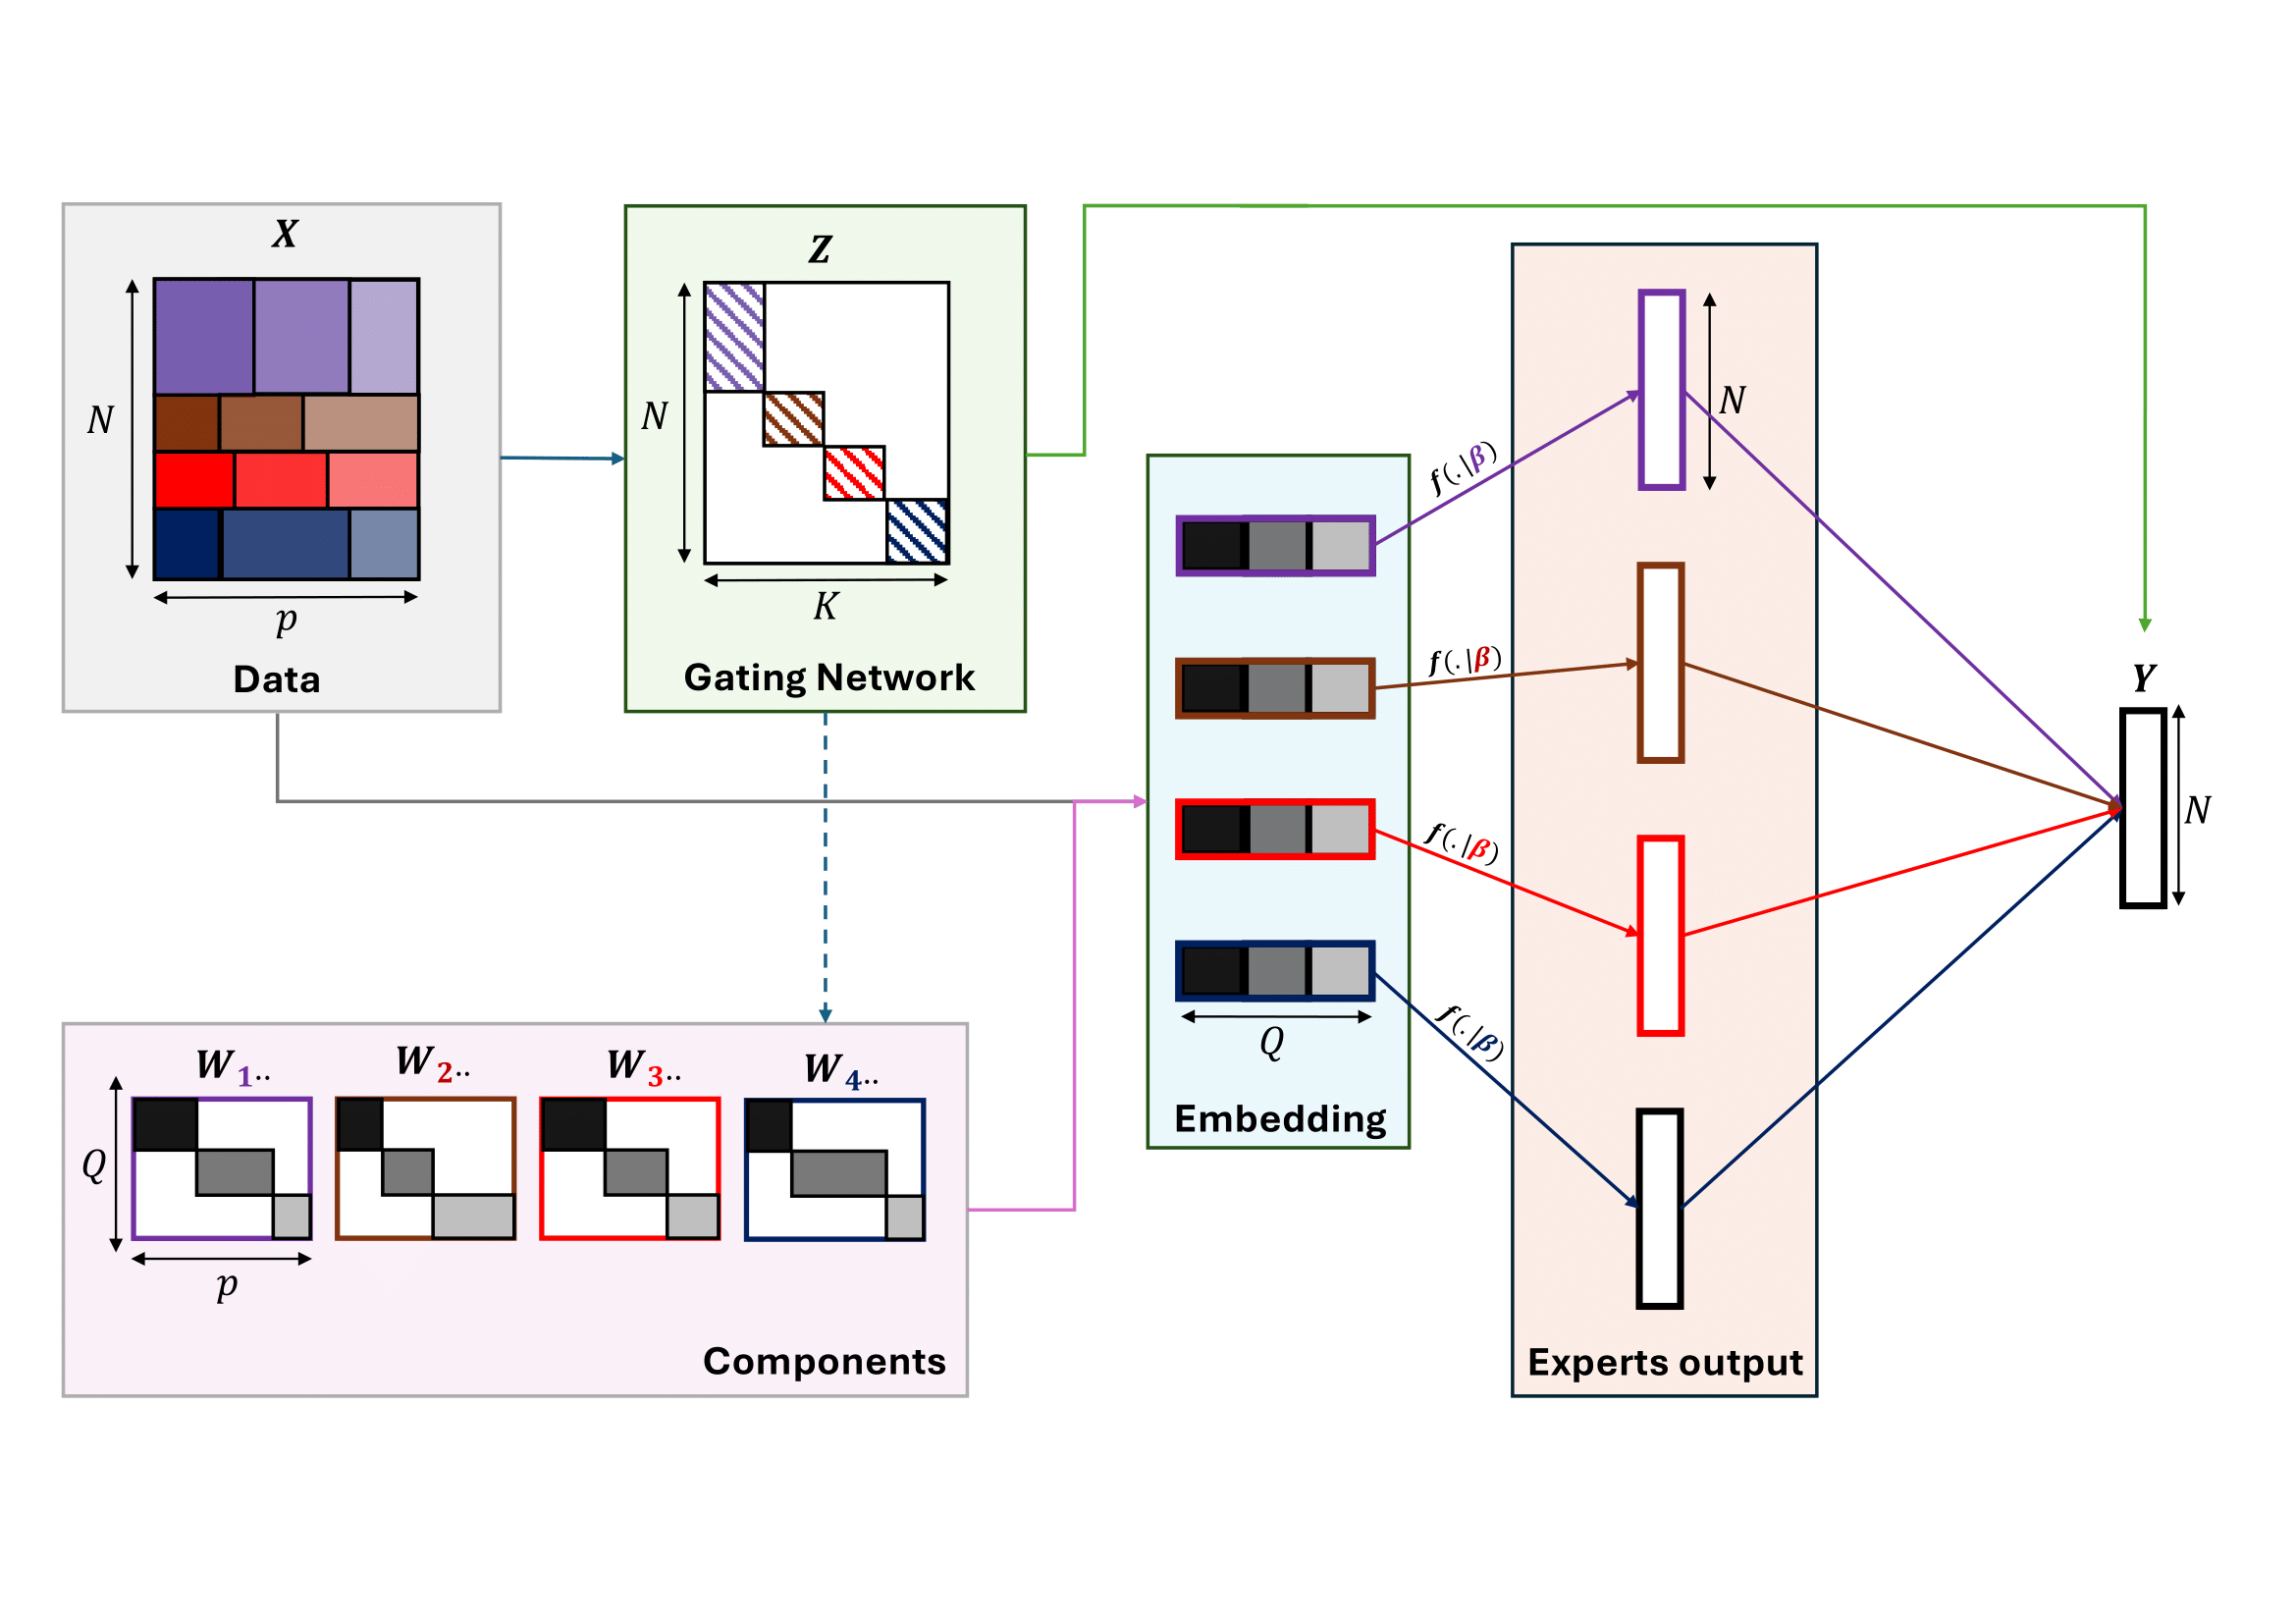
\includegraphics[width=\textwidth]{Figures/CocoLBMoE.png}
     \end{subfigure}
     \hfill
     \caption{ Schematic representation of \textit{MoEBIUS}.
     The input data \( \bX \), of dimension \( N \times p \), is used to define selection weights for the $K$ experts (gating network $\bZ$, with $K$ communities).
     Each expert is associated with a projection matrix \( \bW_k \), of dimension \( p \times Q \), that groups the covariates into components. The data, coupled with the projection matrices, are transformed into matrices of size \( N \times Q \), which are then passed through a regression function \( f_k(. \mid \bbeta_k) \) specific to each expert. 
     The outputs of the experts are combined according to the gating network's weights (based on community membership) to produce a final prediction \( \by \), representing the target variable.}
     \label{fig: CocoLBMoE}
\end{figure}

In modeling the response variable $\by$ conditionally on covariates $\bX$ and latent variables $\bZ$ and $\bW$, different strategies can be employed depending on the nature of the response variable's support.
In this chapter, we focus on two primary settings: regression for continuous outcomes and multinomial logistic regression for categorical outcomes.

\paragraph{Regression} When the support of $\by$ lies in $\mathbb{R}^N$, we adopt the following regression model:
\begin{equation}
y_i \mid \bX_i, Z_{ik} = 1, \bW_{k} \sim \mathcal{N}\left(y_i; \bX_i \bW_{k} \bbeta_k, \sigma^2_k \right) .
\label{eq: reg_CCLBM} 
\end{equation}
In this formulation, the regression parameters $\bbeta_k \in \mathbb{R}^Q$ for each latent class $k$ must be estimated, and $\sigma^2_k$, representing the class-specific noise variance, too.

\paragraph{Multinomial logistic regression} For the case where the support of $\by$ is $\left\{1, \dots, C\right\}^N$, we use a multinomial logistic regression type model:
%
\begin{equation} 
y_i \mid \bX_i, Z_{ik} = 1, \bW_{k} \sim \M\left(1; \softmax\left( \bX_i \bW_{k} \bbeta_k \right)\right).
\label{eq: classif_CCLBM} 
\end{equation}
In this case, the classification parameters $\bbeta_k \in \mathbb{R}^{Q \times C}$ are parameter matrices corresponding to each latent class $k$.

For a given community \( k \), this model can be interpreted as a regression on the vector \( (\bX_i \bW_{k }) \in \mathbb{R}^Q \). The components of this vector represent synthesized features of individual \( i \), conditioned on the partition of community \( k \), and reduced to \( Q \) variables. In other words, the \( p \) original variables are summarized into \( Q \) representative variables, each corresponding to a specific component. The graphical representation of the proposed model is provided in Figure \ref{fig: MoEBIUS Rep Graphique}.
%
\begin{figure}[!ht]
     \centering
     \begin{subfigure}[b]{\textwidth}
         \centering
         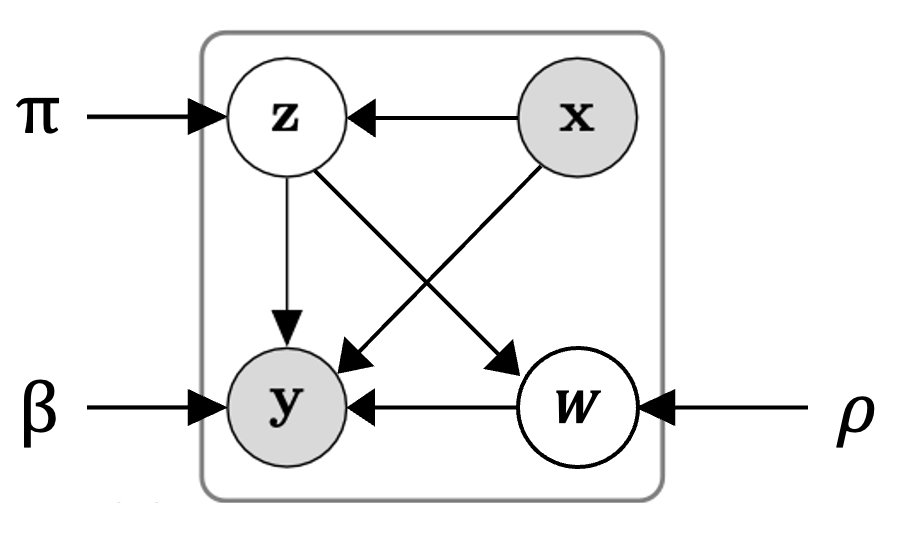
\includegraphics[width=0.6\textwidth]{Figures/CocoLBMoE_repres.png}
     \end{subfigure}
     \hfill
     \caption{Graphical model for \textit{MoEBIUS}. The joint distribution can be factorized as follows:\newline $\p(\by,\bZ,\bW \mid \bX,\bpi, \brho, \bbeta) = \p(\by \mid \bX,\bZ,\bW, \bbeta) \p(\bW \mid \bZ, \brho) \p(\bZ \mid \bX,\bpi)$.}
     \label{fig: MoEBIUS Rep Graphique}
\end{figure}

The complete likelihood can be expressed as:
%
\begin{align}
    \mathcal{L}^c\left(\bbeta, \brho, \bpi; \by,\bZ,\bW \mid \bX\right) &= \p\left(\by,\bZ,\bW \mid \bX, \bpi, \brho, \bbeta   \right) \notag \\
    &= \prod_{i=1}^N \prod_{k=1}^K \p\left(y_i \mid \bZ_{i k},\bW_{k},\bX_i, \bbeta_k   \right)
    \prod_{k=1}^K \prod_{j=1}^p \p\left(\bW_{kj} \mid \bZ,  \brho \right) \notag \\
    &\quad \prod_{i=1}^N  \p\left(\bZ_{i} \mid  \bX_i, \bpi   \right).
\end{align}
% Now, when modeling the target variable $\by$ conditionally on covariates $\bX$ and latent variables $\bZ, \bW$, the problem can be approached in various ways depending on the support of $\by$.

% In this work, we focus on two approaches: regression and multiclass classification.

% \paragraph{Regression}
% Assuming that the support of $\by$ is $\mathbb{R}^N$, we model the target as follows:

% \begin{equation}
%     y_i \mid \bX_i, Z_{ik} = 1 , \bW_{k\bullet\bullet} \sim  \mathcal{N}\left(y_i; \bX_i  \bW_{k\bullet\bullet} \bbeta_k, \sigma^2_k \right)
%     \label{eq: reg_CCLBM}
% \end{equation}

% Here, the regression parameters $(\bbeta_k)_{k=1:K}$ are vectors in $\mathbb{R}^Q$ that need to be estimated.

% \paragraph{Multiclass Classification}
% Assuming that the support of $\by$ is $\left\{1,\dots,C \right\}^N$, we model the target as follows:

% \begin{equation}
%     y_i \mid \bX_i, Z_{ik} = 1 , \bW_{k\bullet\bullet} \sim \M\left(y_i; \softmax\left( \bX_i  \bW_{k\bullet\bullet} \bbeta_k \right) \right)
%     \label{eq: classif_CCLBM}
% \end{equation}

% Here, the classification parameters $(\bbeta_k)_{k=1:K}$ are matrices in $\mathbb{R}^{Q \times C}$ that need to be estimated.



% Thus, the complete likelihood can be written as:

% \begin{align}
%     \mathcal{L}^c\left(\bTheta ; \by,\bZ,\bW \mid \bX\right) &= \p\left(\by,\bZ,\bW \mid \bX, \bTheta   \right) \notag \\
%     &= \prod_{i=1}^N \prod_{k=1}^K \p\left(y_i \mid \bZ_{ik},\bW_{k\bullet \bullet},\bX_i, \bbeta_k   \right)
%     \prod_{k=1}^K \prod_{j=1}^p \p\left(\bW_{kj} \mid \bZ_{ik},  \brho \right) \notag \\
%     &\quad \prod_{i=1}^N  \p\left(\bZ_i \mid  \bX_i, \bpi   \right)
% \end{align}



\subsection{Model Selection}

The model selection process for \textit{MoEBIUS} is based on the ICL criterion proposed by \cite{goffinet2020conditional} for conditional co-clustering and the BIC criterion introduced by \cite{schwarz1978estimating} to penalize the regression component.

\begin{align}
    \operatorname{BIC\_ICL}(\by, \bX,K,Q) =& \log \p \left(\by,\hat{\bZ},\hat{\bW} \mid \bX,  \hat{\bpi}, \hat{\brho}, \hat{\bbeta} \right) 
    - p \dfrac{K-1}{2} \log \left( N \right) \notag \\
    &\quad - K \dfrac{Q-1}{2} \log \left( p \right) 
    - \dfrac{O_{prob}}{2} \log\left(N\right),
\end{align}

where $O_{prob}$ represents the number of parameters depending on the type of model used for $\by$.

The criterion penalizes the log-likelihood based on the number of free parameters, thus preventing overfitting:
\begin{itemize}
    \item For communities $\bpi$: $p \times (K-1)$ free parameters.
    \item For components $\brho$: $K \times (Q-1)$ free parameters.
    \item For regression $\bbeta$: $O_{prob} = 2 \times K \times Q$ free parameters.
    \item For multiclass classification $\bbeta$: $O_{prob} = (C-1) \times K \times Q$ free parameters.
\end{itemize}

The best model is the one that maximizes the BIC\_ICL criterion, achieving a balance between predictive performance and model complexity.

% References
\bibliography{references}

\appendix


\section{Optimization via SEM-Gibbs algorithm}

The Variational EM, as applied in the \textit{mimiSBM} model (Section \ref{sec: VEM_mimiSBM_freq}), is not utilized in this context due to the increased computational complexity. This complexity stems from the dependency between the latent variables forming the tensor $\bW$, which is introduced by the regression component.

However, Gibbs sampling EM emerges as a viable alternative. This approach relies on sampling from the conditional distributions of each variable given the others, which, in our case, are known. This makes Gibbs sampling a practical and implementable strategy for optimizing the model while managing the latent structure effectively.

Through a stochastic EM formulation based on Gibbs sampling, we can estimate latent variables and model parameters for Latent Block Models \citep{keribin2012model}. Moreover, Gibbs sampling is a widely used Monte Carlo Markov Chain method for Bayesian inference in complex statistical models \citep{gelfand1990illustration, yildirim2012bayesian, tobin2024co}. 

As in classical EM algorithms, this optimization consists of two steps: the \textit{ Stochastic Expectation Gibbs-sampling step} (SE-Gibbs step) and the \textit{Maximization step} (M step).
%
We begin by defining the objective function to be optimized at each iteration of the algorithm:
\begin{equation}
    \mathcal{J}\left(\bpi, \brho, \bbeta \mid \bpi^{(t)}, \brho^{(t)}, \bbeta^{(t)} \right) = \mathbb{E}_{\bZ,\bW \sim \p\left(. \mid \by, \bX, \bpi^{(t)}, \brho^{(t)}, \bbeta^{(t)} \right)} \left[ \log \p \left(\by,\bZ,\bW \mid \bX, \bpi, \brho, \bbeta  \right)\right].
\end{equation}


\subsection{Gibbs-sampling Expectation step}
At step (t) of the algorithm, in Gibbs-sampling Expectation step, we first compute the following probabilities:
\begin{equation}
    \tau_{ik}^{(t+1)} = \dfrac{\dfrac{e^{\bX_i \bpi^{(t)}_{\bullet k}}}{\sum_{k'} e^{\bX_i \bpi^{(t)}_{\bullet k'}}} \p\left( y_i \mid \bX_i, Z_{ik}=1,\hat{\bW}^{(t)}_{k }, \bbeta^{(t)}_k\right) }
    {\sum_{k'} \dfrac{e^{\bX_i \bpi^{(t)}_{\bullet k'}}}{\sum_{l} e^{\bX_i \bpi^{(t)}_{\bullet l}}} \p\left( y_i \mid \bX_i,Z_{ik'}=1,\hat{\bW}^{(t)}_{k' }, \bbeta^{(t)}_{k'}\right)},
\label{eq: MoEBIUS_tau}
\end{equation}
with $\bpi_{\bullet k} = \left( \pi_{ik} \right)_{i=1:N}$.

Next, we perform a random draw from a multinomial distribution:
\begin{equation}
    \hat{\bZ}^{(t+1)}_{i} \sim \M\left(1; \left(\tau^{(t+1)}_{i1},\dots,\tau^{(t+1)}_{iK}\right) \right).
\end{equation}

Similarly, the same operations are applied to $\boldsymbol{\nu}$ and $\bW$:
\begin{equation}
    \nu_{kjs}^{(t+1)} = \dfrac{\rho_{ks}^{(t)} \prod_i^N \p\left(y_i \mid \bX_i,\hat{Z}^{(t+1)}_{ik},W_{kjs}=1,\hat{\bW}^{(t)}_{-kj}, \bbeta^{(t)}_k\right)^{\hat{Z}^{(t+1)}_{ik}} }{\sum_{s'} \rho_{ks'}^{(t)} \prod_i^N \p\left(y_i \mid \bX_i,\hat{Z}^{(t+1)}_{ik},W_{kjs'}=1,\hat{\bW}^{(t)}_{-kj}, \bbeta^{(t)}_k\right)^{\hat{Z}^{(t+1)}_{ik}}},
    \label{eq: MoEBIUS_nu}
\end{equation}
where the tensor $\hat{\bW}^{(t)}_{-kj}$ corresponds to tensor $\hat{\bW}^{(t)}$ with the third dimension element associated with the $k$-th entry of the first dimension and the $j$-th entry of the second removed.
%
\begin{equation}
    \hat{\bW}^{(t+1)}_{kj} \sim \M\left(1; \left(\nu^{(t+1)}_{kj1},\dots,\nu^{(t+1)}_{kjQ}\right) \right).
\end{equation}
%
\subsection{Maximization step}
Using the results from the SE-Gibbs step, we now estimate the model parameters $\bpi, \brho, (\bbeta_k)_{k=1:K}$.

For the component parameters $\brho$, The estimation follows a natural approach, where, conditionally on community $k$, the estimation is based on counting the number of variables within the component $s$ and dividing by the total number of variables $p$.
%the estimation is almost identical to that obtained in the optimization of the \textit{Co-coLBM} (Equation \ref{eq: rho_CocoLBM}).
\begin{align}
    \rho_{ks}^{(t+1)} &= \dfrac{\sum_{j=1}^p \hat{\bW}_{kjs}^{(t+1)}}{p},  &\forall k \in \{1,\dots,K\},\forall s \in \{1,\dots,Q\}.
    \label{eq: MoEBIUS_rho}
\end{align}

The parameters $\bpi$ and $(\bbeta_k)_{k=1:K}$ (for multiclass classification) are estimated using a gradient ascent approach, where a step is performed at each iteration of the \textit{SEM-gibbs} algorithm.

Regarding the logistic regression parameters $\bpi$ on the latent variables $(\bZ_i)_{i=1:N}$:
\begin{equation}
    \fracpartial{\mathcal{J}}{\bpi}\left(\bpi, \brho, \bbeta \mid \bpi^{(t)}, \brho^{(t)}, \bbeta^{(t)} \right) = \bX^T \left( \hat{\bZ}^{(t+1)} - \mathbf{S}^{\bpi^{(t)}} \right),
    \label{eq: MoEBIUS_pi}
\end{equation}
with
\begin{equation}
    S^{\bpi}_{ik} = \dfrac{e^{\bX_i \bpi_{\bullet k}}}{\sum_{k'} e^{\bX_i \bpi_{\bullet k'}}}.
\end{equation}

Here, $\hat{\bZ}^{(t+1)}$ represents the "true" community membership matrix, while $\mathbf{S}^{\bpi}$ is an estimate. In other words, the parameters $\bpi$ are optimized to produce predictions consistent with the posterior.

The parameters are updated as follows:
\begin{equation}
    \bpi^{(t+1)} =  \bpi^{(t)} + h_t  \fracpartial{\mathcal{J}}{\bpi}\left(\bpi, \brho, \bbeta \mid \bpi^{(t)}, \brho^{(t)}, \bbeta^{(t)} \right),
\end{equation}
where $h_t$ is the gradient ascent step size for iteration $t$.

The estimation of parameters $(\bbeta_k)_{k=1:K}$ depends on the problem at hand.

\paragraph{Regression}
The estimation of $(\bbeta_k)_{k=1:K}$ is given by:
\begin{equation}
    \bbeta^{(t+1)}_{k} =  \left( {W_{k }^{(t+1)}}^T \bX^T \operatorname{diag}\left(\hat{\bZ}^{(t+1)}_{\bullet k}\right) \bX \bW^{(t+1)}_{k } \right)^{-1}  {\bW^{(t+1)}_{k }}^T \bX^T \operatorname{diag}\left(\hat{\bZ}^{(t+1)}_{\bullet k}\right) \by,
    \label{eq: MoEBIUS_beta_reg}
\end{equation}
with $\hat{\bZ}^{(t+1)}_{\bullet k} = \left( \hat{\bZ}^{(t+1)}_{ik} \right)_{i=1:N}$.
This is a weighted least squares estimator, where the weighting is provided by $\hat{\bZ}^{(t+1)}_{\bullet k}$ and the data matrix is $\bX \bW^{(t+1)}_{k }$.

The estimation of $(\sigma_k^2)_{k=1:K}$ is given by:
\begin{equation}
    {\sigma_k^2}^{(t+1)} = \dfrac{\sum_{i=1}^N \hat{Z}^{(t+1)}_{ik}\left(y_i - \bX_i \hat{\bW}_{k }^{(t+1)}  \bbeta_k^{(t+1)} \right)^2}{\sum_{i=1}^N \hat{Z}^{(t+1)}_{ik}}.
    \label{eq: MoEBIUS_sigma_reg}
\end{equation}

Once again, we find the weighted least squares estimator for ${\sigma_k^2}$.

\paragraph{Multiclass Classification}
The update for the parameters $(\bbeta_k)_{k=1:K}$ is defined as:
\begin{equation}
    \bbeta^{(t+1)}_k =  \bbeta^{(t)}_k + h_t \frac{\partial \mathcal{J}}{\partial \bbeta_k}\left(\bpi, \brho, \bbeta \mid \bpi^{(t)}, \brho^{(t)}, \bbeta^{(t)} \right),
\end{equation}
where the gradient is given by:
\begin{equation}
    \frac{\partial \mathcal{J}}{\partial \bbeta_k} \left(\bpi, \brho, \bbeta \mid \bpi^{(t+1)}, \brho^{(t+1)}, \bbeta^{(t)} \right) = \left[\left( \bX \hat{\bW}^{(t+1)}_{k }\right)^T \odot \mathbf{1}_{Q,1} \hat{\bZ}_{\bullet k}^{(t+1)^T} \right] \left( \by - \mathbf{S}^{\bbeta_k^{(t)}} \right),
    \label{eq: MoEBIUS_beta_classif}
\end{equation}
with the probability of variable $y_i$ belonging to class $c$, for community $k$ and given observation $\bX_i$, defined as:
\begin{equation}
    S^{\bbeta_k}_{ic} = \dfrac{e^{\bX_i \hat{\bW}^{(t+1)}_{k } \bbeta_{k\bullet c}}}{\sum_{c'} e^{\bX_i \hat{\bW}^{(t+1)}_{k } \bbeta_{k\bullet c'}} }.
\end{equation}

Here, $\mathbf{1}_{Q,1}$ is a matrix of size $Q \times 1$ filled with ones,$\odot$ represents the Hadamard (element-wise) product and $\bbeta_{k\bullet c} = \left( \bbeta_{ksc}\right)_{s=1:Q}$.






\end{document}



\endinput
%%
%% End of file `elsarticle-template-num.tex'.
